\chapter{RESULT ANALYSIS}\label{sec4}
\vspace{-3em}

\section{Dataset Design}\label{subsubsec:dataset}

The final evaluation dataset is \texttt{VBRI\_merged.json}, a 352-turn stress-test conversation derived from five real LMSYS-Chat-1M conversations~\cite{zheng2024lmsyschat} produced by vicuna-13b, alpaca-13b, and koala-13b. Each source conversation was first transformed into a replayable hierarchical script with explicit topic labels, subchat actions, selected-text spans, and required response-prefix labels. The final benchmark then merges these five scripts into a single interleaved conversation.

\textbf{Variable-Block Randomized Interleaving (VBRI).}
To stress-test context isolation and recall under realistic multi-topic switching patterns, we developed a merged evaluation scenario using Variable-Block Randomized Interleaving (VBRI). VBRI simulates sessions where users return to earlier topics after short bursts of unrelated discussion while preserving the temporal logic of each original conversation.

The VBRI algorithm operates as follows:
\begin{enumerate}
    \item \textbf{Source-Level FIFO:} Each of the five source scenarios maintains a local queue of ordered blocks. On each iteration, the algorithm selects one source scenario and removes the next block from that source's queue. This guarantees that the original temporal order within every source conversation is preserved.
    \item \textbf{Variable Blocks:} Consecutive same-topic turns are grouped into blocks. Blocks longer than $b_{\max}{=}4$ are split into smaller ordered sub-blocks, preserving short local coherence while preventing one topic from dominating the merged stream.
    \item \textbf{Temporal Preservation:} Within each source scenario, turns maintain their original sequential order. This preserves logical dependencies (e.g., follow-up questions must appear after their referents) while allowing cross-scenario interleaving.
    \item \textbf{Topic Return Dynamics:} With probability $p_{\text{ret}}{=}0.3$, the next block is drawn from the same source as the previous block; otherwise, another active source is selected uniformly. This creates bursty topic revisitation rather than complete random shuffling.
    \item \textbf{Deterministic Reproducibility:} A fixed random seed (42) ensures identical interleaving across experimental runs.
\end{enumerate}

The resulting merged dataset contains 309 original conversation turns spanning 59 distinct LMSYS-derived topics. It contains 91 topic switches, 64 source-conversation switches, 25 topic returns, and no temporal-order violations within any source conversation.

\textbf{Summarization Probes.}
After the 309 ordinary turns, the dataset appends 43 summarization-probe steps, producing 352 total steps. These probes are added only for topics with at least three user turns. Each probe asks the model to summarize what was discussed about one topic, for example: \texttt{Summarize everything we have discussed about ai chat tools. Include all key points, details, and questions that were raised.} The purpose is to test topic-level context retention after a long interleaved conversation, not only immediate topic-prefix selection. In the linear baseline, every probe is sent to the same main conversation node, where all topics have been mixed into one shared history. In Subchat Trees, probes are routed to the relevant topic subchat branch , so the model retrieves from a branch whose local buffer, summary, and vector memory are focused on one topic. This design directly tests whether dividing roles across topic-specific nodes improves the model's ability to recall earlier information.

\textbf{Dataset Structure.}
The dataset is encoded as a JSON file with the following schema:
\begin{itemize}
    \item \texttt{scenario\_name}: Unique identifier for the scenario.
    \item \texttt{conversations}: Ordered list of conversation steps.
    \item Each step contains:
    \begin{itemize}
        \item \texttt{step}: Integer turn number (1-indexed).
        \item \texttt{context}: Ground-truth topic label (e.g., \texttt{``indian\_history''}, \texttt{``astrology''}).
        \item \texttt{message}: Raw user query.
        \item \texttt{node\_type}: Target subchat identifier (e.g., \texttt{``main''}, \texttt{``subchat\_indian\_history''}).
        \item \texttt{action}: Operation type (\texttt{create\_subchat}, \texttt{switch\_node}, or implicit continuation).
        \item \texttt{selected\_text}: (Optional) Text fragment selected for follow-up subchat creation.
        \item \texttt{subchat\_title}: (Optional) Human-readable title for new subchats.
        \item \texttt{parent\_node\_type}: (Optional) Parent node for hierarchical subchat creation.
        \item \texttt{is\_recall\_probe}: (Optional) Boolean marker for appended summarization-probe steps.
        \item \texttt{probe\_topic}: (Optional) Topic being tested by a summarization probe.
        \item \texttt{probe\_target\_node}: (Optional) Target node for a summarization probe.
    \end{itemize}
\end{itemize}

For example, a step from the merged interleaved dataset:
\begin{verbatim}
{
  "step": 45,
  "context": "indian_legal_family",
  "message": "Can you explain the Hindu Succession Act?",
  "node_type": "subchat_indian_legal_family",
  "action": "create_subchat",
  "selected_text": "Indian legal framework",
  "subchat_title": "Hindu Succession Act Discussion",
  "parent_node_type": "subchat_indian_legal"
}
\end{verbatim}

This structure enables deterministic replay: the test harness iterates through steps sequentially, performs the specified action (create subchat, switch node), sends the user message to the target node, and scores the response against the ground-truth context label.

Summarization probes use the same replay mechanism. They are encoded as \texttt{switch\_node} steps so the baseline can ask the probe in its single main node, while Subchat Trees can ask the same probe in the topic-specific node indicated by \texttt{probe\_target\_node}. Probe responses are excluded from topic-prefix isolation counts and are used only for recall scoring.

In the baseline condition, all steps are replayed into one linear conversation node (MAIN) regardless of their annotated \texttt{node\_type}. In the Subchat Trees condition, \texttt{create\_subchat} steps instantiate child nodes under the annotated parent, \texttt{switch\_node} steps route the next message to an existing node, and ordinary continuation steps remain in the current annotated node. This means both conditions receive the same user messages in the same order; only the context organization differs.

Table~\ref{tab:scenarios} summarizes the dataset provenance using the original LMSYS conversation identifiers. The table reports the five source conversations that form \texttt{merged\_vbri\_temporal}, the final dataset used in the Kaggle run.

\begin{table}[htbp]
\caption{Conversation-level provenance for the final VBRI dataset. Turns denote replay turns contributed to \texttt{merged\_realistic\_interleaved.json}, excluding appended recall probes.}\label{tab:scenarios}
\centering
\scriptsize
\setlength{\tabcolsep}{4pt}
\begin{tabular*}{\textwidth}{@{\extracolsep\fill}p{3.2cm}ccp{6.0cm}@{}}
\toprule
\textbf{Source Conversation ID} & \textbf{Turns} & \textbf{Topics} & \textbf{Source Stress Pattern} \\
\midrule
\texttt{22807e655dd04}\newline\texttt{2348cb0ee402}\newline\texttt{3672e70} & 52 & 4 & Persona roleplay, role reversal, LLM-knowledge questions, and Twenty Questions game-state confusion \\
\texttt{6c4992f0aed04}\newline\texttt{dd3bf9a4bc225}\newline\texttt{bb4fb0} & 62 & 11 & Medical discussion, AI consciousness, repetitive-loop failure, pandemic safety, and literature analysis \\
\texttt{8d10c143f8fc4}\newline\texttt{a7599a5a1877}\newline\texttt{8fec112} & 77 & 17 & DSP, C programming, medical genetics, Linux audio, physics, science fiction, geography, and games \\
\texttt{eaf06f12a1d74}\newline\texttt{e5ca30a7ca94}\newline\texttt{a7c4128} & 53 & 8 & Cookie recipes, recipe-halving math errors, argumentative correction, jokes, and emoji game turns \\
\texttt{ec366fd3e4b54}\newline\texttt{82e8acac750f}\newline\texttt{9b3b55b} & 64 & 19 & Explicit context resets across Indian history, LSAT reasoning, law, nutrition, astrology, travel, therapy, and chess \\
\midrule
\textbf{\texttt{merged\_vbri\_temporal}} & \textbf{309} & \textbf{59} & \textbf{Final interleaved benchmark used for context-isolation scoring and recall probes} \\
\botrule
\end{tabular*}
\end{table}

The final replay contains 309 ordinary conversation turns and 59 normalized topic labels. Its replay annotations create 51 subchats. The probe-injected version appends 43 recall probes, producing 352 total steps; those probes are not counted as ordinary conversation turns in Table~\ref{tab:scenarios}.

\section{Evaluation Matrices}\label{subsubsec:metrics}

The evaluation reports four complementary matrices. Each matrix measures a different part of the study: whether a conversation system can keep the right topic active, retain the content of that topic, how  efficiently the system is and can we reduce retrieval rate.

\textbf{Context Isolation Matrix.}
The context isolation matrix measures turn-level topic control. For each ordinary replay turn $t$, the dataset provides a ground-truth topic label $\tau_t$. The model response is scored by extracting the leading topic prefix, denoted $\hat{\tau}_t$. A turn is correct when $\hat{\tau}_t=\tau_t$; otherwise it is counted as context pollution because the response has been assigned to the wrong conversational context. This metric therefore evaluates both memory of the active topic and the ability to match the user query to the correct topic state.

For each topic $\tau_i$, we build a one-vs-rest confusion matrix:
\begin{itemize}
    \item $\text{TP}_i$: $\tau_i$ was expected and the response was labeled as $\tau_i$.
    \item $\text{FP}_i$: another topic was expected, but the response was labeled as $\tau_i$.
    \item $\text{FN}_i$: $\tau_i$ was expected, but the response was labeled as another topic or as unknown.
\end{itemize}
The support $n_i$ is the number of turns whose ground-truth topic is $\tau_i$. Per-topic precision, recall, and F1 are:
\begin{equation}
P_i = \frac{\text{TP}_i}{\text{TP}_i + \text{FP}_i}, \quad
R_i = \frac{\text{TP}_i}{\text{TP}_i + \text{FN}_i}, \quad
F1_i = \frac{2P_iR_i}{P_i + R_i}.
\label{eq:per_topic_metrics}
\end{equation}
The main table reports support-weighted averages:
\begin{equation}
\text{Precision}_w = \sum_i \frac{n_i}{\sum_j n_j} P_i, \quad
\text{Recall}_w = \sum_i \frac{n_i}{\sum_j n_j} R_i, \quad
\text{F1}_w = \sum_i \frac{n_i}{\sum_j n_j} F1_i.
\label{eq:weighted_isolation}
\end{equation}
Macro averages are also computed by giving every topic equal weight. Weighted scores show performance over the full replay distribution, while macro scores check whether improvements are not limited to high-frequency topics.

Overall accuracy and pollution rate are computed over all ordinary replay turns:
\begin{equation}
\text{Accuracy} = \frac{|\{t:\hat{\tau}_t=\tau_t\}|}{N}, \quad
\text{Pollution Rate} = 1-\text{Accuracy},
\label{eq:accuracy_pollution}
\end{equation}
where $N$ is the number of ordinary replay turns. A lower pollution rate means fewer responses were contaminated by another topic.

\textbf{Topic Recall Matrix.}
The topic recall matrix evaluates content retention rather than only topic-label selection. After the 309 ordinary replay turns, the dataset adds summarization probes for every topic with at least three user turns. Each probe asks the model to summarize what was discussed about one topic:
\begin{equation}
\operatorname{Probe}(\tau_i) = \textsc{SummarizeTopic}(\tau_i).
\label{eq:probe}
\end{equation}
For each probed topic, the reference trace $R_i$ is built from the user messages and assistant responses that occurred under that topic during the same evaluation run. The model's generated summary $S_i$ is compared with $R_i$ using ROUGE-1 F1, ROUGE-L F1, and BLEU-2:
\begin{equation}
\text{Recall}^{m} = \frac{1}{|\mathcal{P}|}\sum_{\tau_i \in \mathcal{P}} m(S_i, R_i),
\label{eq:recall_probe_agg}
\end{equation}
where $\mathcal{P}$ is the set of 43 probed topics and $m$ is one of the three overlap metrics. ROUGE-1 measures unigram content overlap, ROUGE-L measures ordered sequence overlap, and BLEU-2 measures short phrase overlap~\cite{lin2004rouge,papineni2002bleu}. These probes are relevant because a system may output the correct topic prefix while still failing to recover the earlier details of that topic.

In the baseline, all recall probes are asked in the same main node after the full interleaved conversation. The model must therefore recover one topic from a mixed history. In SubchatTrees, probes are routed to the corresponding topic branch when such a branch exists. Since each branch stores a more focused local buffer, summary, and vector memory, the recall matrix directly tests whether topic-specific structure improves long-range retention.

\textbf{System Performance Matrix.}
The system performance matrix measures the operational cost of producing correct answers. For each ordinary replay turn, we record input tokens, output tokens, total tokens, and latency. The average total-token cost is:
\begin{equation}
\overline{T}_{\text{total}} = \frac{1}{N}\sum_{t=1}^{N} T_t.
\label{eq:avg_tokens}
\end{equation}
Token compression compares the average total tokens used by Subchat Trees against the linear baseline:
\begin{equation}
\text{Token Compression} = \frac{\overline{T}_{\text{baseline}}-\overline{T}_{\text{SubchatTrees}}}{\overline{T}_{\text{baseline}}}\times100\%.
\label{eq:compression}
\end{equation}
Because a cheaper answer is not useful if it is wrong, we also report tokens per correct answer:
\begin{equation}
\text{Tokens Per Correct Answer} = \frac{\sum_{t=1}^{N} T_t}{|\{t:\hat{\tau}_t=\tau_t\}|}.
\label{eq:tpca}
\end{equation}
This combines context accuracy and token use into one efficiency measure. Cost per query is estimated from average input and output tokens:
\begin{equation}
\text{Cost Per Query} = \frac{\overline{T}_{\text{in}}p_{\text{in}}+\overline{T}_{\text{out}}p_{\text{out}}}{10^6},
\label{eq:cost}
\end{equation}
where $p_{\text{in}}$ and $p_{\text{out}}$ are prices per million input and output tokens.

\textbf{RAG Decision Matrix.}
The RAG decision matrix measures how often the system needs to leave the active buffer and retrieve archived context. For every RAG-eligible turn, the retrieval controller returns either \textit{search triggered} or \textit{buffer sufficient}. Let $N_{\text{rag}}$ be the number of eligible turns, $N_{\text{search}}$ the number of turns that triggered retrieval, and $N_{\text{buffer}}$ the number of turns handled by the recent buffer. We report:
\begin{equation}
\text{Retrieval Rate} = \frac{N_{\text{search}}}{N_{\text{rag}}}\times100\%, \quad
\text{Buffer Rate} = \frac{N_{\text{buffer}}}{N_{\text{rag}}}\times100\%.
\label{eq:rag_rates}
\end{equation}
This matrix is relevant because retrieval behavior reflects context locality. In a flat transcript, the active buffer often contains unrelated topics, so the model may need archived retrieval to recover the relevant history. In Subchat Trees, each subchat contains information related mainly to its own topic. A lower retrieval rate together with higher isolation or recall therefore indicates that the system is relying less on archive search because the active branch already contains more relevant context.

\section{Topic-Scoring Pipeline}\label{subsubsec:classify}

All scripted evaluation turns require the model to start its answer with the active topic label followed by a colon. The primary isolation score therefore uses deterministic prefix extraction rather than a subjective semantic judge. This choice makes the metric reproducible and intentionally strict: a response that discusses the correct content but begins with the wrong topic label is counted as polluted because the system failed to preserve conversational state.

\begin{algorithm}[htbp]
\caption{Deterministic Topic-Prefix Scoring}\label{alg:classify}
\begin{algorithmic}[1]
\Require Response $r$, expected topic $\tau$, valid topic set $\mathcal{T}$
\Ensure Correctness flag $y \in \{0,1\}$ and detected topic $\hat{\tau}$
\State $\hat{\tau} \gets \textsc{RegexExtractPrefix}(r)$ \Comment{First token sequence before ``:''}
\If{$\hat{\tau} \in \mathcal{T}$ \textbf{and} $\hat{\tau} = \tau$}
    \State \Return $(1, \hat{\tau})$
\Else
    \State \Return $(0, \hat{\tau})$
\EndIf
\end{algorithmic}
\end{algorithm}

For non-introductory turns, the scorer extracts the response prefix using a regular expression of the form \texttt{\^{}([a-zA-Z\_][a-zA-Z0-9\_]*)\textbackslash s*:}. If the extracted prefix equals the normalized ground-truth topic, the turn is counted as correct; otherwise it contributes a false negative for the expected topic and, when applicable, a false positive for the detected topic. Introductory acknowledgement turns are scored only for non-empty completion and are excluded from topic-prefix matching. An LLM-based judge module is retained in the codebase for diagnostic analysis, but the reported isolation tables use the deterministic prefix scorer.

% 
% For each scenario, model scale, and buffer size $C \in \{5, 10, 20, 40\}$:
% \begin{enumerate}
%     \item Run the linear baseline from a clean server state (fresh ChromaDB).
%     \item Run the Subchat Trees system from a clean server state.
%     \item Score all responses using deterministic topic-prefix extraction and compute per-topic metrics.
% \end{enumerate}

% \textbf{Reproducibility.} Deterministic decoding for evaluation runs, deterministic topic-prefix scoring, vector-store clearing between tests, version-controlled JSON scenario files, and the single-notebook Kaggle harness ensure full reproducibility. Output length is capped during inference to standardize response length across conditions.

%%==================================%%
%% SECTION 4: RESULTS              %%
%%==================================%%
The final evaluation compares a linear-chat baseline against Subchat Trees on the same 309-turn VBRI Dataset. The system evaluate Qwen2.5 7B, 14B, and 32B AWQ models at buffer sizes $C \in \{5,10,20,40\}$. The ordinary replay turns measure topic isolation through deterministic prefix scoring. After those turns, 43 recall probes ask the model to summarize prior discussion for each sufficiently frequent topic. This section is organized model by model because the most important result is not a single global score, but how model capacity changes the useful buffer range, retrieval behavior, and failure mode.

\section{How to Read the Result Tables}\label{subsec:reading_results}

% The topic-isolation task uses a deliberately strict instruction. The model is told that each new topic is introduced with a pattern such as \texttt{topic\_name : user query}, and that every answer must start with the active topic name followed by a colon. The key instruction is:


The topic-isolation task uses a deliberately strict instruction. The model is told that each new topic starts with a pattern such as \texttt{topic\_name : user query}, and every reponse from the LLM active topic name followed by a colon. The key instruction was:


\begin{verbatim}
REQUIRED FORMAT for EVERY response:
Start your answer with the active topic or sub-topic name,
followed by a colon, then give your actual answer.
\end{verbatim}

This matters because Table~1 isolation metrics are not semantic relevance scores. A response can discuss the right content and still be counted as polluted if it starts with the wrong topic prefix or no prefix at all. This strict scoring is useful for testing conversational state control. it can also exposes instruction-following limits in smaller models.


On the other hand, The 43 recall probes use a different measurement. For each eligible topic, the probe asks:

\begin{verbatim}
Summarize everything we have discussed about {topic}. Include all
key points, details, and questions that were raised.
\end{verbatim}

% These probes are excluded from topic-prefix F1 and are reported through ROUGE-1, ROUGE-L, BLEU-2, probe token cost, and probe RAG decisions. In the baseline, every probe is asked in the single linear node. In Subchat Trees, probes are routed to the relevant topic branch when available. Therefore, recall probes test whether the system can recover topic content after long interleaving, while isolation F1 tests whether it can keep the active topic label correct during ordinary turns.


These probes are not included in topic-prefix F1 score. Instead, they are evaluated using ROUGE-1, ROUGE-L, BLEU-2, probe token cost, and probe RAG decisions. For baseline every probe is asked in a single linear node. In SubchatTrees, probles are routed in their relevent branch. Thus, recall probes measures weither the system can recover topic content after a long interleaving Conversation.On the other hand, isolation F1 tests whether it can correctly classify topic labels based on user query.





\section{7B Model: Context Structure Helps, but Instruction Following Remains Fragile}\label{subsec:results_7b}

% The 7B model exposes the hardest operating regime. Subchat Trees improves the linear baseline at every buffer size, but the model remains fragile as the prompt grows. Table~\ref{tab:7b_context_main} shows that system F1 is highest at $C=5$ (62.9\%) and then falls to 55.2\%, 45.6\%, and 39.3\% as the buffer grows. The baseline collapses more severely, reaching only 9.8\% F1 at $C=40$. This is a model-capacity problem as much as a memory problem: the small model has difficulty preserving a hidden formatting rule after many turns, summaries, and retrieved snippets.




The 7B model expose the hardest operating regime. SubchatTrees surplus the baseline at every buffer setting, but the model remains fragile as the context grows. From Table~\ref{tab:7b_context_main} it can be observed that system F1 is highest at $C=5$ (62.9\%). As buffer size increases both system and baselien performance decreases 55.2\%, 45.6\%, and 39.3\%. The baseline even collapses more severely reaching 9.8\% F1 at $C=40$. This is a model specific problem rather than a memory problem. The small model struggle preserving a formatting rule after many turns, as context grows exponentially larger. This is a limitation of the 7B model to follow instruction.




\begin{table}[htbp]
\caption{7B: merged context-isolation metrics across buffer sizes.}\label{tab:7b_context_main}
\centering
\scriptsize
\setlength{\tabcolsep}{3pt}
\begin{adjustbox}{width=\textwidth}
\begin{tabular}{lcccccccc}
\toprule
\textbf{Metric} & \multicolumn{2}{c}{\textbf{Buffer 5}} & \multicolumn{2}{c}{\textbf{Buffer 10}} & \multicolumn{2}{c}{\textbf{Buffer 20}} & \multicolumn{2}{c}{\textbf{Buffer 40}} \\
\cmidrule(lr){2-3}\cmidrule(lr){4-5}\cmidrule(lr){6-7}\cmidrule(lr){8-9}
 & \textbf{Base} & \textbf{System} & \textbf{Base} & \textbf{System} & \textbf{Base} & \textbf{System} & \textbf{Base} & \textbf{System} \\
\midrule
Precision & 44.7\% & 84.0\% & 71.5\% & 88.7\% & 34.9\% & 80.7\% & 21.5\% & 76.2\% \\
Recall & 21.1\% & 58.1\% & 39.6\% & 46.1\% & 15.6\% & 38.3\% & 7.8\% & 33.4\% \\
F1 & 24.3\% & 62.9\% & 44.7\% & 55.2\% & 18.7\% & 45.6\% & 9.8\% & 39.3\% \\
Accuracy & 21.4\% & 58.3\% & 39.8\% & 46.3\% & 15.9\% & 38.5\% & 8.1\% & 33.7\% \\
Pollution Rate & 78.6\% & 41.7\% & 60.2\% & 53.7\% & 84.1\% & 61.5\% & 91.9\% & 66.3\% \\
Macro Precision & 48.5\% & 74.4\% & 70.9\% & 85.6\% & 41.7\% & 76.0\% & 29.0\% & 72.8\% \\
Macro Recall & 33.7\% & 59.6\% & 49.4\% & 59.7\% & 24.7\% & 50.5\% & 17.8\% & 41.4\% \\
Macro F1 & 35.2\% & 60.8\% & 53.6\% & 65.3\% & 27.2\% & 55.6\% & 19.0\% & 46.5\% \\
\botrule
\end{tabular}
\end{adjustbox}
\end{table}

% The recall table changes the interpretation of the low 7B F1 scores. Table~\ref{tab:7b_recall_main} shows that the tree system retains substantially more topic content than the baseline even when prefix compliance degrades. At $C=20$, ROUGE-1 rises from 0.1811 to 0.4056, ROUGE-L rises from 0.1016 to 0.3194, and BLEU-2 rises from 0.0205 to 0.1325. In other words, the branch structure is preserving useful semantic material, but the 7B model cannot always turn that material into a correctly prefixed answer.




The recall table changes the interpretation of the low 7B F1 scores. Table~\ref{tab:7b_recall_main} shows that the tree system retains more topic content than the baseline. At $C=20$ ROUGE-1 rises from 0.1811 to 0.4046 double context retention, ROUGE-L rises from 0.1016 to 0.3194 and BLEU-2 rises from 0.0205 to 0.1325. In other words, the subchat system is preserving more useful semantic material than the baseline.





\begin{table}[htbp]
\caption{7B: aggregate recall-probe scores and probe cost. Topic-specific rows are kept in the appendix; this table reports the major aggregate recall results.}\label{tab:7b_recall_main}
\centering
\scriptsize
\setlength{\tabcolsep}{3pt}
\begin{adjustbox}{width=\textwidth}
\begin{tabular}{lcccccccc}
\toprule
\textbf{Metric} & \multicolumn{2}{c}{\textbf{Buffer 5}} & \multicolumn{2}{c}{\textbf{Buffer 10}} & \multicolumn{2}{c}{\textbf{Buffer 20}} & \multicolumn{2}{c}{\textbf{Buffer 40}} \\
\cmidrule(lr){2-3}\cmidrule(lr){4-5}\cmidrule(lr){6-7}\cmidrule(lr){8-9}
 & \textbf{Base} & \textbf{System} & \textbf{Base} & \textbf{System} & \textbf{Base} & \textbf{System} & \textbf{Base} & \textbf{System} \\
\midrule
Avg ROUGE-1 (F1) & 0.2448 & 0.4240 & 0.2369 & 0.4094 & 0.1811 & 0.4056 & 0.1557 & 0.3545 \\
Avg ROUGE-L (F1) & 0.1270 & 0.3004 & 0.1349 & 0.3097 & 0.1016 & 0.3194 & 0.0861 & 0.2574 \\
Avg BLEU-2 & 0.0364 & 0.1581 & 0.0324 & 0.1259 & 0.0205 & 0.1325 & 0.0172 & 0.1142 \\
Topics Probed & 43 & 43 & 43 & 43 & 43 & 43 & 43 & 43 \\
Total Probe Tokens & 158,043 & 121,521 & 252,519 & 188,722 & 336,942 & 284,817 & 472,634 & 403,852 \\
Avg Tokens per Probe & 3,675 & 2,826 & 5,873 & 4,389 & 7,836 & 6,624 & 10,991 & 9,392 \\
Total Probe Latency & 918.00s & 710.28s & 814.85s & 776.91s & 767.61s & 792.74s & 723.47s & 703.08s \\
Avg Probe Latency & 21.35s & 16.52s & 18.95s & 18.07s & 17.85s & 18.44s & 16.82s & 16.35s \\
\botrule
\end{tabular}
\end{adjustbox}
\end{table}

% The performance Table~\ref{tab:7b_recall_main} also shows why raw token count alone is not the right story. At $C=5$, the system uses fewer average input tokens than baseline, but at larger buffers system input becomes slightly larger. This does not contradict the architecture. The logs show that disorganized baseline context often produces short, generic, or incorrectly prefixed answers, while branch-local context gives the model enough relevant evidence to answer more fully. The better efficiency signal is tokens per correct answer: Subchat Trees lowers this metric at every 7B buffer size, including 35,451 to 15,389 at $C=20$ and 102,923 to 25,899 at $C=40$.




The performance Table~\ref{tab:7b_recall_main} shows that the system uses more average input token than the baseline. Further, observing the logs reveal that disorganized baseline context often produces short, generic response. In contrast, Subchat system provides enough context to the model to answer more confidently and fully. This behavior can increase token count. Where suchat provides more detailed and confident response and baseline provide safe and short response. At $C=10 to 40$ subchat system input becoming slightly larger than the baseline. A better efficiency measurement would be token used per correct answer: SubchatTrees lowers this metrics at every buffer size, including 35,451 to 15,389 at $C=20$ and at $C=40$ 102,923 to 25,899





\begin{table}[htbp]
\caption{7B: merged system-performance metrics, including recall/summarization probe token accounting.}\label{tab:7b_perf_main}
\centering
\tiny
\setlength{\tabcolsep}{2.2pt}
\begin{adjustbox}{width=\textwidth}
\begin{tabular}{lcccccccc}
\toprule
\textbf{Metric} & \multicolumn{2}{c}{\textbf{Buffer 5}} & \multicolumn{2}{c}{\textbf{Buffer 10}} & \multicolumn{2}{c}{\textbf{Buffer 20}} & \multicolumn{2}{c}{\textbf{Buffer 40}} \\
\cmidrule(lr){2-3}\cmidrule(lr){4-5}\cmidrule(lr){6-7}\cmidrule(lr){8-9}
 & \textbf{Base} & \textbf{System} & \textbf{Base} & \textbf{System} & \textbf{Base} & \textbf{System} & \textbf{Base} & \textbf{System} \\
\midrule
Normal Conversation Turns & 309 & 309 & 309 & 309 & 309 & 309 & 309 & 309 \\
Avg Input Tokens & 2,270 & 2,205 & 3,384 & 3,556 & 5,386 & 5,685 & 8,107 & 8,487 \\
Avg Output Tokens & 205 & 164 & 214 & 235 & 235 & 241 & 220 & 230 \\
Avg Total Tokens & 2,476 & 2,369 & 3,598 & 3,791 & 5,622 & 5,927 & 8,327 & 8,717 \\
Total Tokens & 765,017 & 732,147 & 1,111,680 & 1,171,373 & 1,737,082 & 1,831,296 & 2,573,086 & 2,693,481 \\
Tokens Per Correct Answer & 11,591 & 4,067 & 9,038 & 8,191 & 35,451 & 15,389 & 102,923 & 25,899 \\
Avg Latency & 12.19s & 10.14s & 10.62s & 10.55s & 11.70s & 11.22s & 11.75s & 11.71s \\
Cost per Query & \$0.000130 & \$0.000123 & \$0.000186 & \$0.000197 & \$0.000288 & \$0.000304 & \$0.000423 & \$0.000443 \\
Summarization Probe Calls & 43 & 43 & 43 & 43 & 43 & 43 & 43 & 43 \\
Summarization Probe Tokens & 158,043 & 121,521 & 252,519 & 188,722 & 336,942 & 284,817 & 472,634 & 403,852 \\
Avg Tokens per Summarization Probe & 3,675 & 2,826 & 5,873 & 4,389 & 7,836 & 6,624 & 10,991 & 9,392 \\
Combined Evaluated Calls & 352 & 352 & 352 & 352 & 352 & 352 & 352 & 352 \\
Combined Total Tokens & 923,060 & 853,668 & 1,364,199 & 1,360,095 & 2,074,024 & 2,116,113 & 3,045,720 & 3,097,333 \\
Combined Avg Tokens per Call & 2,622 & 2,425 & 3,876 & 3,864 & 5,892 & 6,012 & 8,653 & 8,799 \\
\botrule
\end{tabular}
\end{adjustbox}
\end{table}

The 7B recall-probe RAG table should be read as a retrieval-calibration failure. During recall probes, the system triggers RAG more than the baseline at every buffer size. At $C=5$, system probe retrieval is 39.5\% while baseline probe retrieval is only 2.3\%. This is not the expected memory-sufficiency pattern; it suggests the smaller model is unsure whether branch-local context is enough and overuses retrieval despite stronger recall scores. Or toll using capability is limited for this smaller version

\begin{table}[htbp]
\caption{7B: merged recall/summarization-probe RAG decision breakdown.}\label{tab:7b_rag_main}
\centering
\tiny
\setlength{\tabcolsep}{2.2pt}
\begin{adjustbox}{width=\textwidth}
\begin{tabular}{lcccccccc}
\toprule
\textbf{Metric} & \multicolumn{2}{c}{\textbf{Buffer 5}} & \multicolumn{2}{c}{\textbf{Buffer 10}} & \multicolumn{2}{c}{\textbf{Buffer 20}} & \multicolumn{2}{c}{\textbf{Buffer 40}} \\
\cmidrule(lr){2-3}\cmidrule(lr){4-5}\cmidrule(lr){6-7}\cmidrule(lr){8-9}
 & \textbf{Base} & \textbf{System} & \textbf{Base} & \textbf{System} & \textbf{Base} & \textbf{System} & \textbf{Base} & \textbf{System} \\
\midrule
Probe Turns & 43 & 43 & 43 & 43 & 43 & 43 & 43 & 43 \\
RAG-Eligible Probe Turns & 43 & 43 & 43 & 43 & 43 & 43 & 43 & 43 \\
Probe RAG Triggered & 1 & 17 & 2 & 9 & 2 & 4 & 0 & 1 \\
Probe Buffer Sufficient & 42 & 26 & 41 & 34 & 41 & 39 & 43 & 42 \\
Probe Retrieval Rate & 2.3\% & 39.5\% & 4.7\% & 20.9\% & 4.7\% & 9.3\% & 0.0\% & 2.3\% \\
Probe Buffer Rate & 97.7\% & 60.5\% & 95.3\% & 79.1\% & 95.3\% & 90.7\% & 100.0\% & 97.7\% \\
Probe Errors & 0 & 0 & 0 & 0 & 0 & 0 & 0 & 0 \\
\botrule
\end{tabular}
\end{adjustbox}
\end{table}

Overall, the 7B finding is clear: the SubChat architecture improves memory and reduces pollution. Here the main limiting factor was a small model not being able to handle tool calling or follow instruction. The architecture helps, but it cannot fully compensate for weak instruction following.

\section{14B Model: The Cleanest Practical Tradeoff}\label{subsec:results_14b}

% The 14B model provides the clearest evidence for the architecture. Table~\ref{tab:14b_context_main} shows that system F1 improves from 73.9\% at $C=5$ to 83.4\% at $C=10$ and 83.1\% at $C=20$. The drop to 73.1\% at $C=40$ is important: it shows that increasing the buffer is not automatically beneficial. At $C=40$, summarization happens later, leaving more raw user and assistant turns in the prompt together with summaries, system instructions, and possible retrieval context. The result is not simply more memory; it is a heavier prompt that can overwhelm the model.





The 14B model provides the clearest evidence for the architecture. Table~\ref{tab:14b_context_main} shows that system F1 improves from 73.9\% at $C=5$ to 83.4\% at $C=10$ and 83.1\% at $C=20$. The drop at $C=40$ to 73.1\% is also architecturally significant. It shows that increasing the buffer is not automatically beneficial. At $C=40$ summarization happens later, leaving more raw user and assistant turns in the prompt along with long rolling summaries, system instructions and possible retrieval context. The result is not simply more memory, it is a heavier context that can easily overwhelm the model.


\begin{table}[htbp]
\caption{14B: merged context-isolation metrics across buffer sizes.}\label{tab:14b_context_main}
\centering
\scriptsize
\setlength{\tabcolsep}{3pt}
\begin{adjustbox}{width=\textwidth}
\begin{tabular}{lcccccccc}
\toprule
\textbf{Metric} & \multicolumn{2}{c}{\textbf{Buffer 5}} & \multicolumn{2}{c}{\textbf{Buffer 10}} & \multicolumn{2}{c}{\textbf{Buffer 20}} & \multicolumn{2}{c}{\textbf{Buffer 40}} \\
\cmidrule(lr){2-3}\cmidrule(lr){4-5}\cmidrule(lr){6-7}\cmidrule(lr){8-9}
 & \textbf{Base} & \textbf{System} & \textbf{Base} & \textbf{System} & \textbf{Base} & \textbf{System} & \textbf{Base} & \textbf{System} \\
\midrule
Precision & 64.5\% & 77.8\% & 81.2\% & 93.2\% & 85.0\% & 89.2\% & 81.6\% & 85.3\% \\
Recall & 52.6\% & 74.4\% & 59.7\% & 80.2\% & 60.1\% & 81.8\% & 55.8\% & 69.5\% \\
F1 & 51.2\% & 73.9\% & 64.3\% & 83.4\% & 62.5\% & 83.1\% & 59.8\% & 73.1\% \\
Accuracy & 52.8\% & 74.4\% & 59.9\% & 80.3\% & 60.2\% & 81.9\% & 56.0\% & 69.6\% \\
Pollution Rate & 47.2\% & 25.6\% & 40.1\% & 19.7\% & 39.8\% & 18.1\% & 44.0\% & 30.4\% \\
Macro Precision & 52.0\% & 67.5\% & 75.7\% & 88.1\% & 77.6\% & 85.4\% & 73.4\% & 79.5\% \\
Macro Recall & 52.7\% & 68.5\% & 67.3\% & 78.7\% & 65.4\% & 79.5\% & 61.8\% & 65.3\% \\
Macro F1 & 48.3\% & 65.8\% & 67.1\% & 80.1\% & 65.1\% & 79.7\% & 61.4\% & 67.9\% \\
\botrule
\end{tabular}
\end{adjustbox}
\end{table}

The recall-probe table shows the same pattern from the memory side. System ROUGE-1 remains around 0.42 at $C=10$ and $C=20$, while baseline ROUGE-1 keeps droping from 0.3378 at $C=10$ to 0.2476 at $C=20$ and 0.1745 at $C=40$. This is fall indicates that baseline is not only forgetting, it is mixing unrelated context. The tree system keeps the relevant branch recoverable.

\begin{table}[htbp]
\caption{14B: aggregate recall-probe scores and probe cost.}\label{tab:14b_recall_main}
\centering
\scriptsize
\setlength{\tabcolsep}{3pt}
\begin{adjustbox}{width=\textwidth}
\begin{tabular}{lcccccccc}
\toprule
\textbf{Metric} & \multicolumn{2}{c}{\textbf{Buffer 5}} & \multicolumn{2}{c}{\textbf{Buffer 10}} & \multicolumn{2}{c}{\textbf{Buffer 20}} & \multicolumn{2}{c}{\textbf{Buffer 40}} \\
\cmidrule(lr){2-3}\cmidrule(lr){4-5}\cmidrule(lr){6-7}\cmidrule(lr){8-9}
 & \textbf{Base} & \textbf{System} & \textbf{Base} & \textbf{System} & \textbf{Base} & \textbf{System} & \textbf{Base} & \textbf{System} \\
\midrule
Avg ROUGE-1 (F1) & 0.3428 & 0.3896 & 0.3378 & 0.4201 & 0.2476 & 0.4187 & 0.1745 & 0.3725 \\
Avg ROUGE-L (F1) & 0.2179 & 0.2634 & 0.1982 & 0.3211 & 0.1320 & 0.3143 & 0.0997 & 0.2648 \\
Avg BLEU-2 & 0.0967 & 0.1099 & 0.0870 & 0.1338 & 0.0516 & 0.1237 & 0.0182 & 0.1315 \\
Topics Probed & 43 & 43 & 43 & 43 & 43 & 43 & 43 & 43 \\
Total Probe Tokens & 136,045 & 104,023 & 274,209 & 156,136 & 322,902 & 269,171 & 359,355 & 304,196 \\
Avg Tokens per Probe & 3,164 & 2,419 & 6,377 & 3,631 & 7,509 & 6,260 & 8,357 & 7,074 \\
Total Probe Latency & 1155.49s & 989.76s & 1441.58s & 997.15s & 1284.58s & 1196.07s & 943.70s & 957.29s \\
Avg Probe Latency & 26.87s & 23.02s & 33.53s & 23.19s & 29.87s & 27.82s & 21.95s & 22.26s \\
\botrule
\end{tabular}
\end{adjustbox}
\end{table}

The 14B performance table gives the practical tradeoff. Raw input tokens are not always lower for the system, especially at $C=20$ and $C=40$, but tokens per correct answer are lower at every buffer size. At $C=20$, the baseline sends 8,036 tokens per correct answer while the system spends 6,853. At $C=40$, the baseline sends 10,418 while the system sends 8,826 token. Considering correctness subchat system is more efficient than the baseline linear system.














\begin{table}[htbp]
\caption{14B: merged system-performance metrics, including recall/summarization probe token accounting.}\label{tab:14b_perf_main}
\centering
\tiny
\setlength{\tabcolsep}{2.2pt}
\begin{adjustbox}{width=\textwidth}
\begin{tabular}{lcccccccc}
\toprule
\textbf{Metric} & \multicolumn{2}{c}{\textbf{Buffer 5}} & \multicolumn{2}{c}{\textbf{Buffer 10}} & \multicolumn{2}{c}{\textbf{Buffer 20}} & \multicolumn{2}{c}{\textbf{Buffer 40}} \\
\cmidrule(lr){2-3}\cmidrule(lr){4-5}\cmidrule(lr){6-7}\cmidrule(lr){8-9}
 & \textbf{Base} & \textbf{System} & \textbf{Base} & \textbf{System} & \textbf{Base} & \textbf{System} & \textbf{Base} & \textbf{System} \\
\midrule
Normal Conversation Turns & 309 & 309 & 309 & 309 & 309 & 309 & 309 & 309 \\
Avg Input Tokens & 1,818 & 1,919 & 3,152 & 3,092 & 4,659 & 5,396 & 5,685 & 5,981 \\
Avg Output Tokens & 133 & 145 & 170 & 182 & 177 & 215 & 148 & 160 \\
Avg Total Tokens & 1,952 & 2,064 & 3,321 & 3,274 & 4,837 & 5,611 & 5,833 & 6,141 \\
Total Tokens & 603,033 & 637,814 & 1,026,292 & 1,011,686 & 1,494,607 & 1,733,862 & 1,802,333 & 1,897,579 \\
Tokens Per Correct Answer & 3,700 & 2,773 & 5,548 & 4,079 & 8,036 & 6,853 & 10,418 & 8,826 \\
Avg Latency & 16.71s & 16.16s & 15.00s & 13.58s & 16.06s & 17.69s & 14.58s & 14.64s \\
Cost per Query & \$0.000102 & \$0.000108 & \$0.000171 & \$0.000169 & \$0.000247 & \$0.000287 & \$0.000296 & \$0.000312 \\
Summarization Probe Calls & 43 & 43 & 43 & 43 & 43 & 43 & 43 & 43 \\
Summarization Probe Tokens & 136,045 & 104,023 & 274,209 & 156,136 & 322,902 & 269,171 & 359,355 & 304,196 \\
Avg Tokens per Summarization Probe & 3,164 & 2,419 & 6,377 & 3,631 & 7,509 & 6,260 & 8,357 & 7,074 \\
Combined Evaluated Calls & 352 & 352 & 352 & 352 & 352 & 352 & 352 & 352 \\
Combined Total Tokens & 739,078 & 741,837 & 1,300,501 & 1,167,822 & 1,817,509 & 2,003,033 & 2,161,688 & 2,201,775 \\
Combined Avg Tokens per Call & 2,100 & 2,107 & 3,695 & 3,318 & 5,163 & 5,690 & 6,141 & 6,255 \\
\botrule
\end{tabular}
\end{adjustbox}
\end{table}

From the RAG table, During recall probes, baseline retrieval is high at small buffers and then decreases as the buffer grows: 58.1\%, 44.2\%, 37.2\%, and 16.3\%. The system is much lower: 23.3\%, 2.3\%, 4.7\%, and 0.0\%. This behavior is expected. In the baseline, old topic content is either evicted or buried among unrelated turns, so the model asks for archive retrieval. In the tree system, the active branch often already contains enough local evidence, So the LLM decides not to use retrieval. As buffer size grows for both system and baseline the chances of having sufficient context in buffer increase, thus retrieval decreases.

\begin{table}[htbp]
\caption{14B: merged recall/summarization-probe RAG decision breakdown.}\label{tab:14b_rag_main}
\centering
\tiny
\setlength{\tabcolsep}{2.2pt}
\begin{adjustbox}{width=\textwidth}
\begin{tabular}{lcccccccc}
\toprule
\textbf{Metric} & \multicolumn{2}{c}{\textbf{Buffer 5}} & \multicolumn{2}{c}{\textbf{Buffer 10}} & \multicolumn{2}{c}{\textbf{Buffer 20}} & \multicolumn{2}{c}{\textbf{Buffer 40}} \\
\cmidrule(lr){2-3}\cmidrule(lr){4-5}\cmidrule(lr){6-7}\cmidrule(lr){8-9}
 & \textbf{Base} & \textbf{System} & \textbf{Base} & \textbf{System} & \textbf{Base} & \textbf{System} & \textbf{Base} & \textbf{System} \\
\midrule
Probe Turns & 43 & 43 & 43 & 43 & 43 & 43 & 43 & 43 \\
RAG-Eligible Probe Turns & 43 & 43 & 43 & 43 & 43 & 43 & 43 & 41 \\
Probe RAG Triggered & 25 & 10 & 19 & 1 & 16 & 2 & 7 & 0 \\
Probe Buffer Sufficient & 18 & 33 & 24 & 42 & 27 & 41 & 36 & 41 \\
Probe Retrieval Rate & 58.1\% & 23.3\% & 44.2\% & 2.3\% & 37.2\% & 4.7\% & 16.3\% & 0.0\% \\
Probe Buffer Rate & 41.9\% & 76.7\% & 55.8\% & 97.7\% & 62.8\% & 95.3\% & 83.7\% & 100.0\% \\
Probe Errors & 0 & 0 & 0 & 0 & 0 & 0 & 0 & 2 \\
\botrule
\end{tabular}
\end{adjustbox}
\end{table}

The 14B model therefore supports the main architectural claim most cleanly. Moderate buffers provide enough local context while allowing summarization to compact older turns before the prompt becomes too heavy and noisy. In this setting, Subchat Trees further improves isolation, recall, retrieval efficiency and tokens per correct answer.

\section{32B Model: Strongest Absolute Performance and Better Long-Context Tolerance}\label{subsec:results_32b}

% The 32B model reaches the strongest absolute performance. Table~\ref{tab:32b_context_main} shows that the system is above 83\% F1 from $C=5$ through $C=20$, peaking at 85.2\% at $C=20$. Even at $C=40$, the system remains at 78.2\%, a smaller drop than the 7B and 14B models. This indicates that stronger models can tolerate longer context better, but the system still improves over the baseline at every buffer size.






The 32B model reaches the strongest absolute performance. Table~\ref{tab:32b_context_main} shows that the system is above 83\% F1 at only $C=5$ through $C=20$. The peak score was 85.2\% at $C=20$. Even at $C=40$, the subchat system remains at 78.2\%, a reasonable drop compare to 7B and 14B models. This is expected as we know stronger models can tolerate longer context better, But the SubChat system still outperform baseline at every buffer settings.








\begin{table}[htbp]
\caption{32B: merged context-isolation metrics across buffer sizes.}\label{tab:32b_context_main}
\centering
\scriptsize
\setlength{\tabcolsep}{3pt}
\begin{adjustbox}{width=\textwidth}
\begin{tabular}{lcccccccc}
\toprule
\textbf{Metric} & \multicolumn{2}{c}{\textbf{Buffer 5}} & \multicolumn{2}{c}{\textbf{Buffer 10}} & \multicolumn{2}{c}{\textbf{Buffer 20}} & \multicolumn{2}{c}{\textbf{Buffer 40}} \\
\cmidrule(lr){2-3}\cmidrule(lr){4-5}\cmidrule(lr){6-7}\cmidrule(lr){8-9}
 & \textbf{Base} & \textbf{System} & \textbf{Base} & \textbf{System} & \textbf{Base} & \textbf{System} & \textbf{Base} & \textbf{System} \\
\midrule
Precision & 88.0\% & 88.5\% & 87.3\% & 94.4\% & 89.9\% & 93.4\% & 84.9\% & 90.0\% \\
Recall & 64.6\% & 83.1\% & 69.2\% & 80.2\% & 67.2\% & 83.4\% & 63.6\% & 74.4\% \\
F1 & 68.6\% & 83.2\% & 71.1\% & 83.7\% & 69.6\% & 85.2\% & 65.7\% & 78.2\% \\
Accuracy & 64.7\% & 83.2\% & 69.3\% & 80.3\% & 67.3\% & 83.5\% & 63.8\% & 74.4\% \\
Pollution Rate & 35.3\% & 16.8\% & 30.7\% & 19.7\% & 32.7\% & 16.5\% & 36.2\% & 25.6\% \\
Macro Precision & 83.6\% & 85.1\% & 81.4\% & 91.8\% & 86.7\% & 93.0\% & 78.3\% & 88.2\% \\
Macro Recall & 73.9\% & 81.9\% & 75.2\% & 79.8\% & 75.8\% & 86.8\% & 71.6\% & 74.0\% \\
Macro F1 & 74.4\% & 80.8\% & 73.9\% & 81.9\% & 74.5\% & 87.1\% & 68.4\% & 76.7\% \\
\botrule
\end{tabular}
\end{adjustbox}
\end{table}

The recall metrics \ref{tab:32b_recall_main} are also the strongest for the system so far. At $C=20$ system ROUGE-1 is 0.4283 in compare of 0.3338 for the baseline. As buffer grows, At $C=40$ the baseline collapses to 0.1503 while the system remains at 0.3918. The reduction in baseline recall happened simply because of too much irrelevant context. This is one of the clearest signs that the linear baseline becomes overwhelmed by topic mixture. The Subchat system keeps the relevant branch recoverable.











\begin{table}[htbp]
\caption{32B: aggregate recall-probe scores and probe cost.}\label{tab:32b_recall_main}
\centering
\scriptsize
\setlength{\tabcolsep}{3pt}
\begin{adjustbox}{width=\textwidth}
\begin{tabular}{lcccccccc}
\toprule
\textbf{Metric} & \multicolumn{2}{c}{\textbf{Buffer 5}} & \multicolumn{2}{c}{\textbf{Buffer 10}} & \multicolumn{2}{c}{\textbf{Buffer 20}} & \multicolumn{2}{c}{\textbf{Buffer 40}} \\
\cmidrule(lr){2-3}\cmidrule(lr){4-5}\cmidrule(lr){6-7}\cmidrule(lr){8-9}
 & \textbf{Base} & \textbf{System} & \textbf{Base} & \textbf{System} & \textbf{Base} & \textbf{System} & \textbf{Base} & \textbf{System} \\
\midrule
Avg ROUGE-1 (F1) & 0.2687 & 0.4328 & 0.3674 & 0.4206 & 0.3338 & 0.4283 & 0.1503 & 0.3918 \\
Avg ROUGE-L (F1) & 0.1767 & 0.2830 & 0.2274 & 0.2982 & 0.2009 & 0.3016 & 0.0878 & 0.2624 \\
Avg BLEU-2 & 0.0502 & 0.1452 & 0.1023 & 0.1253 & 0.0731 & 0.1247 & 0.0234 & 0.1206 \\
Topics Probed & 43 & 43 & 43 & 43 & 43 & 43 & 43 & 43 \\
Total Probe Tokens & 119,832 & 131,487 & 249,908 & 175,875 & 373,285 & 264,906 & 324,171 & 310,617 \\
Avg Tokens per Probe & 2,787 & 3,058 & 5,812 & 4,090 & 8,681 & 6,161 & 7,539 & 7,224 \\
Total Probe Latency & 1959.92s & 2495.09s & 2965.46s & 2722.82s & 3002.40s & 2796.51s & 1888.54s & 2288.25s \\
Avg Probe Latency & 45.58s & 58.03s & 68.96s & 63.32s & 69.82s & 65.04s & 43.92s & 53.22s \\
\botrule
\end{tabular}
\end{adjustbox}
\end{table}

The 32B performance table shows the cost of stronger inference, while confirming the same efficiency pattern observed so far. Though The 32B model is slower than the smaller models but Subchat  reduces tokens per correct answer at every buffer size. At $C=20$, the baseline sends 7,775 tokens per correct answer but the system sends 6,600. The system also has lower average latency than baseline at $C=5$, $C=10$, and $C=40$. This indicates organized context can offset some of the cost of richer answers.

\begin{table}[htbp]
\caption{32B: merged system-performance metrics, including recall/summarization probe token accounting.}\label{tab:32b_perf_main}
\centering
\tiny
\setlength{\tabcolsep}{2.2pt}
\begin{adjustbox}{width=\textwidth}
\begin{tabular}{lcccccccc}
\toprule
\textbf{Metric} & \multicolumn{2}{c}{\textbf{Buffer 5}} & \multicolumn{2}{c}{\textbf{Buffer 10}} & \multicolumn{2}{c}{\textbf{Buffer 20}} & \multicolumn{2}{c}{\textbf{Buffer 40}} \\
\cmidrule(lr){2-3}\cmidrule(lr){4-5}\cmidrule(lr){6-7}\cmidrule(lr){8-9}
 & \textbf{Base} & \textbf{System} & \textbf{Base} & \textbf{System} & \textbf{Base} & \textbf{System} & \textbf{Base} & \textbf{System} \\
\midrule
Normal Conversation Turns & 309 & 309 & 309 & 309 & 309 & 309 & 309 & 309 \\
Avg Input Tokens & 2,038 & 2,119 & 3,165 & 3,156 & 5,043 & 5,292 & 6,252 & 6,405 \\
Avg Output Tokens & 139 & 158 & 173 & 176 & 191 & 219 & 162 & 170 \\
Avg Total Tokens & 2,177 & 2,277 & 3,338 & 3,331 & 5,234 & 5,511 & 6,413 & 6,575 \\
Total Tokens & 672,623 & 703,603 & 1,031,367 & 1,029,385 & 1,617,294 & 1,702,877 & 1,981,748 & 2,031,629 \\
Tokens Per Correct Answer & 3,363 & 2,738 & 4,819 & 4,151 & 7,775 & 6,600 & 10,060 & 8,833 \\
Avg Latency & 36.91s & 35.86s & 37.52s & 33.71s & 38.99s & 39.29s & 34.77s & 33.56s \\
Cost per Query & \$0.000113 & \$0.000119 & \$0.000172 & \$0.000172 & \$0.000267 & \$0.000282 & \$0.000326 & \$0.000334 \\
Summarization Probe Calls & 43 & 43 & 43 & 43 & 43 & 43 & 43 & 43 \\
Summarization Probe Tokens & 119,832 & 131,487 & 249,908 & 175,875 & 373,285 & 264,906 & 324,171 & 310,617 \\
Avg Tokens per Summarization Probe & 2,787 & 3,058 & 5,812 & 4,090 & 8,681 & 6,161 & 7,539 & 7,224 \\
Combined Evaluated Calls & 352 & 352 & 352 & 352 & 352 & 352 & 352 & 352 \\
Combined Total Tokens & 792,455 & 835,090 & 1,281,275 & 1,205,260 & 1,990,579 & 1,967,783 & 2,305,919 & 2,342,246 \\
Combined Avg Tokens per Call & 2,251 & 2,372 & 3,640 & 3,424 & 5,655 & 5,590 & 6,551 & 6,654 \\
\botrule
\end{tabular}
\end{adjustbox}
\end{table}

% The 32B RAG behavior is more nuanced than 14B. At $C=5$, the system retrieves more during recall probes than the baseline, suggesting that a short branch-local buffer may not contain enough evidence for full-topic summaries. But once the buffer reaches 10, 20, and 40, system probe retrieval falls below baseline. At $C=40$, baseline probe retrieval is 72.1\% while system probe retrieval is only 2.4\%. The stronger model can use the organized branch context effectively once enough local history is available.




The 32B RAG behavior is more nuanced than the 14B or the 7B model. The system retrieves more during recall probes than the baseline. This suggest a short branch may not contain enough context thus the model decides to use its retrieval tool more often. But as buffer grows 10, 20 and 40, system probe retrieval falls below baseline. At $C=40$ baseline probe retrieval is 72.1\%, meaning it is now more confused with the large mixed context whether the buffer contains relevant information or whether it should search on the vector store with specific keywords that user asked. On the other hand at $C=40$ Subchat retrieval rate is only 2.4\%, indicating the stronger model can use the organized branch context more effectively. 
 




\begin{table}[htbp]
\caption{32B: merged recall/summarization-probe RAG decision breakdown.}\label{tab:32b_rag_main}
\centering
\tiny
\setlength{\tabcolsep}{2.2pt}
\begin{adjustbox}{width=\textwidth}
\begin{tabular}{lcccccccc}
\toprule
\textbf{Metric} & \multicolumn{2}{c}{\textbf{Buffer 5}} & \multicolumn{2}{c}{\textbf{Buffer 10}} & \multicolumn{2}{c}{\textbf{Buffer 20}} & \multicolumn{2}{c}{\textbf{Buffer 40}} \\
\cmidrule(lr){2-3}\cmidrule(lr){4-5}\cmidrule(lr){6-7}\cmidrule(lr){8-9}
 & \textbf{Base} & \textbf{System} & \textbf{Base} & \textbf{System} & \textbf{Base} & \textbf{System} & \textbf{Base} & \textbf{System} \\
\midrule
Probe Turns & 43 & 43 & 43 & 43 & 43 & 43 & 43 & 43 \\
RAG-Eligible Probe Turns & 43 & 43 & 43 & 43 & 43 & 43 & 43 & 42 \\
Probe RAG Triggered & 23 & 38 & 40 & 23 & 26 & 8 & 31 & 1 \\
Probe Buffer Sufficient & 20 & 5 & 3 & 20 & 17 & 35 & 12 & 41 \\
Probe Retrieval Rate & 53.5\% & 88.4\% & 93.0\% & 53.5\% & 60.5\% & 18.6\% & 72.1\% & 2.4\% \\
Probe Buffer Rate & 46.5\% & 11.6\% & 7.0\% & 46.5\% & 39.5\% & 81.4\% & 27.9\% & 97.6\% \\
Probe Errors & 0 & 0 & 0 & 0 & 0 & 0 & 0 & 1 \\
\botrule
\end{tabular}
\end{adjustbox}
\end{table}

The 32B model reveals that The stronger model tolerates larger buffers better, but the tree system still provides a consistent advantage in isolation, recall, pollution reduction and tokens per correct answer.







\section{Cross-Model Visual Synthesis}\label{subsec:cross_model_visuals}

 The following figures summarize the global pattern across models and buffers. The best observed system performances are reflected in Table \ref{tab:best_by_model} The best absolute result is 32B at $C=20$. The 14B at $C=10/20$ provides a strong practical tradeoff. The 7B model shows the largest rescue effect but instruction-following stays limited.

\begin{table}[htbp]
\caption{Best Subchat Trees configuration for each model.}\label{tab:best_by_model}
\centering
\scriptsize
\begin{tabular*}{\textwidth}{@{\extracolsep\fill}lcccccc@{}}
\toprule
\textbf{Model} & \textbf{Best $C$} & \textbf{Base F1} & \textbf{System F1} & \textbf{F1 Gain} & \textbf{Base Pollution} & \textbf{System Pollution} \\
\midrule
7B & 5 & 24.3\% & 62.9\% & +38.6 pts & 78.6\% & 41.7\% \\
14B & 10 & 64.3\% & 83.4\% & +19.1 pts & 40.1\% & 19.7\% \\
32B & 20 & 69.6\% & 85.2\% & +15.7 pts & 32.7\% & 16.5\% \\
\botrule
\end{tabular*}
\end{table}

Figure~\ref{fig:f1_buffer_all} shows context-isolation F1 across all runs. SubchatTrees improves over the baseline in every configuration. The weakest model benefits most in relative terms, while the strongest model reaches the highest absolute performance. SubchatTree shows strong performance, even the 14B Subchat System performs better than the 32B baseline.

\begin{figure}[htbp]
\centering
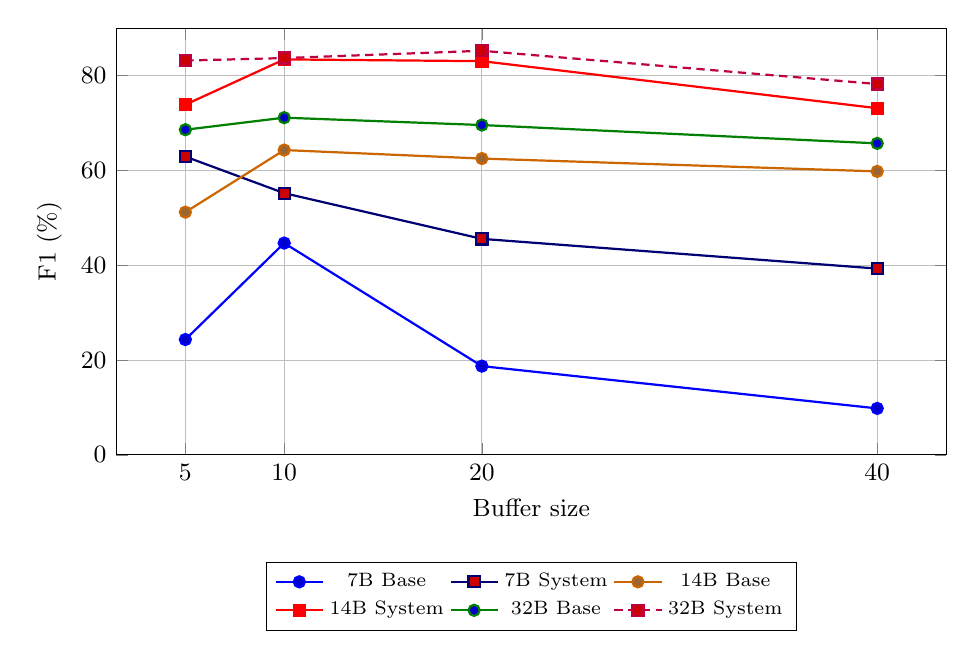
\begin{tikzpicture}
\begin{axis}[
width=\textwidth,
height=7cm,
xlabel={Buffer size},
ylabel={F1 (\%)},
xtick={5,10,20,40},
grid=both,
legend columns=3,
legend style={font=\scriptsize, at={(0.5,-0.25)}, anchor=north},
tick label style={font=\small},
label style={font=\small},
ymin=0,
ymax=90
]
\addplot+[color=blue, mark=*, thick] coordinates {(5,24.3277) (10,44.6750) (20,18.7204) (40,9.8033)};
\addlegendentry{7B Base}
\addplot+[color=blue!45!black, mark=square*, thick] coordinates {(5,62.9179) (10,55.2057) (20,45.5658) (40,39.2950)};
\addlegendentry{7B System}
\addplot+[color=orange!80!black, mark=*, thick] coordinates {(5,51.1988) (10,64.2995) (20,62.5056) (40,59.7974)};
\addlegendentry{14B Base}
\addplot+[color=red, mark=square*, thick] coordinates {(5,73.8736) (10,83.4215) (20,83.0537) (40,73.1313)};
\addlegendentry{14B System}
\addplot+[color=green!50!black, mark=*, thick] coordinates {(5,68.5899) (10,71.1312) (20,69.5766) (40,65.7086)};
\addlegendentry{32B Base}
\addplot+[color=purple, mark=square*, thick] coordinates {(5,83.1796) (10,83.7040) (20,85.2437) (40,78.2294)};
\addlegendentry{32B System}
\end{axis}
\end{tikzpicture}
\caption{Context-isolation F1 across model sizes and buffer sizes. Subchat Trees improves F1 over the linear baseline in every configuration.}
\label{fig:f1_buffer_all}
\end{figure}

Figure~\ref{fig:pollution_buffer_all} gives the matching pollution rate. At $C=20$, pollution falls from 84.1\% to 61.5\% for 7B, for 14B it is from 39.8\% to 18.1\%, and  32.7\% to 16.5\% for 32B. This directly supports that the failure is not only forgetting, but also contamination from unrelated conversational state.

\begin{figure}[htbp]
\centering
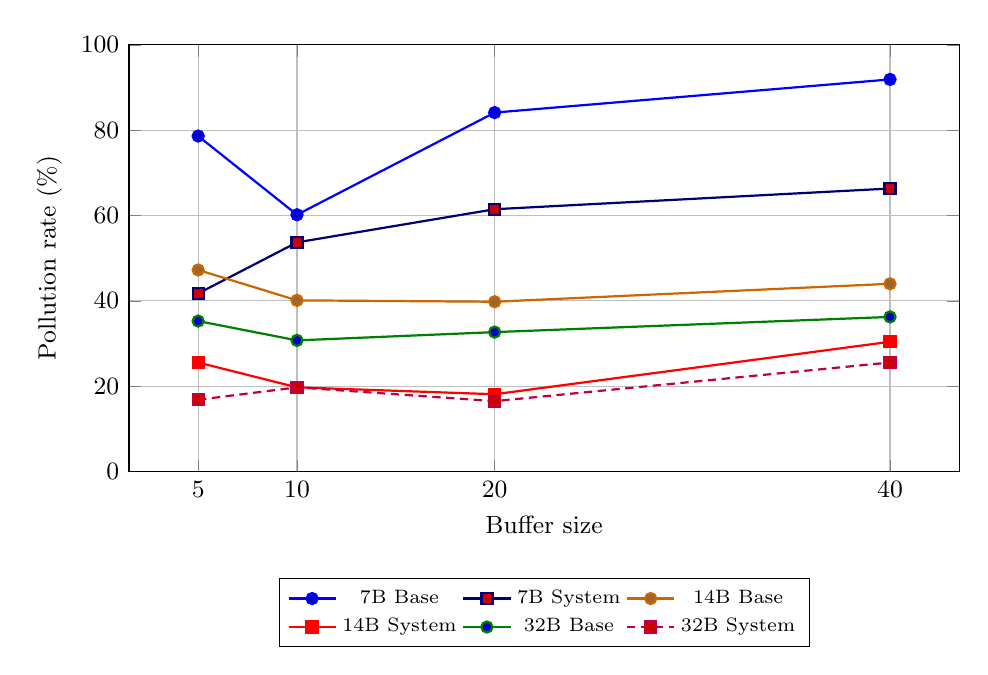
\begin{tikzpicture}
\begin{axis}[
width=\textwidth,
height=7cm,
xlabel={Buffer size},
ylabel={Pollution rate (\%)},
xtick={5,10,20,40},
grid=both,
legend columns=3,
legend style={font=\scriptsize, at={(0.5,-0.25)}, anchor=north},
tick label style={font=\small},
label style={font=\small},
ymin=0,
ymax=100
]
\addplot+[color=blue, mark=*, thick] coordinates {(5,78.6408) (10,60.1942) (20,84.1424) (40,91.9094)};
\addlegendentry{7B Base}
\addplot+[color=blue!45!black, mark=square*, thick] coordinates {(5,41.7476) (10,53.7217) (20,61.4887) (40,66.3430)};
\addlegendentry{7B System}
\addplot+[color=orange!80!black, mark=*, thick] coordinates {(5,47.2492) (10,40.1294) (20,39.8058) (40,44.0129)};
\addlegendentry{14B Base}
\addplot+[color=red, mark=square*, thick] coordinates {(5,25.5663) (10,19.7411) (20,18.1230) (40,30.4207)};
\addlegendentry{14B System}
\addplot+[color=green!50!black, mark=*, thick] coordinates {(5,35.2751) (10,30.7443) (20,32.6861) (40,36.2460)};
\addlegendentry{32B Base}
\addplot+[color=purple, mark=square*, thick] coordinates {(5,16.8285) (10,19.7411) (20,16.5049) (40,25.5663)};
\addlegendentry{32B System}
\end{axis}
\end{tikzpicture}
\caption{Pollution rate across buffer sizes. Lower values are better. Subchat Trees consistently reduces cross-topic contamination by routing turns into branch-local buffers instead of keeping all topics in one linear transcript.}
\label{fig:pollution_buffer_all}
\end{figure}

Figure~\ref{fig:rouge1_buffer_all} summarizes the recall-probe result. The Subchat system improves average ROUGE-1 in every model-buffer setting. This matters because it shows that the tree system is preserving more topic content.

\begin{figure}[htbp]
\centering
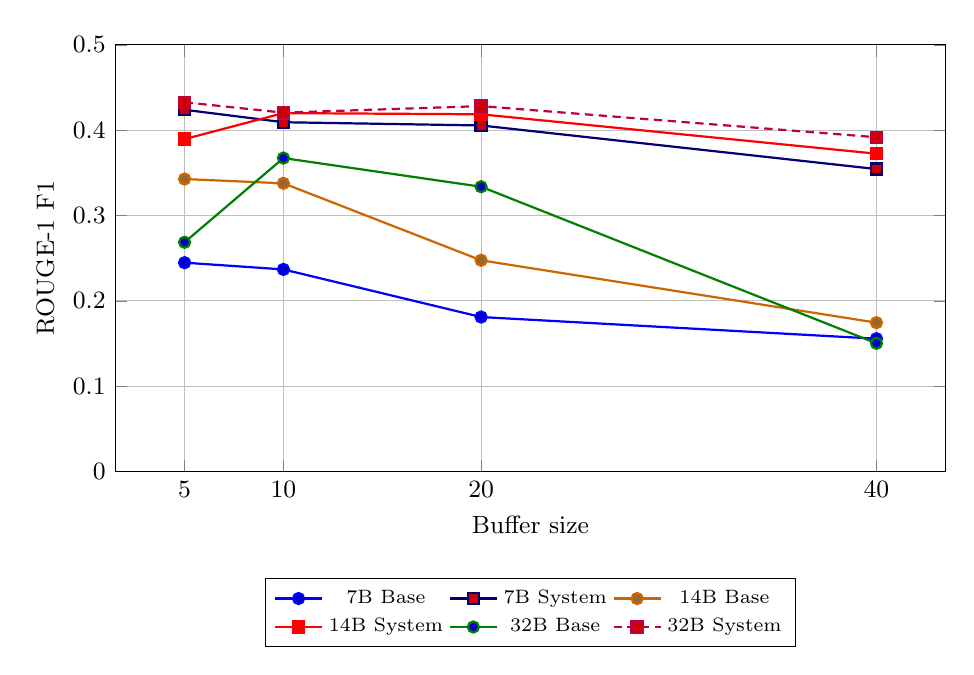
\begin{tikzpicture}
\begin{axis}[
width=\textwidth,
height=7cm,
xlabel={Buffer size},
ylabel={ROUGE-1 F1},
xtick={5,10,20,40},
grid=both,
legend columns=3,
legend style={font=\scriptsize, at={(0.5,-0.25)}, anchor=north},
tick label style={font=\small},
label style={font=\small},
ymin=0,
ymax=0.5
]
\addplot+[color=blue, mark=*, thick] coordinates {(5,0.2448) (10,0.2369) (20,0.1811) (40,0.1557)};
\addlegendentry{7B Base}
\addplot+[color=blue!45!black, mark=square*, thick] coordinates {(5,0.4240) (10,0.4094) (20,0.4056) (40,0.3545)};
\addlegendentry{7B System}
\addplot+[color=orange!80!black, mark=*, thick] coordinates {(5,0.3428) (10,0.3378) (20,0.2476) (40,0.1745)};
\addlegendentry{14B Base}
\addplot+[color=red, mark=square*, thick] coordinates {(5,0.3896) (10,0.4201) (20,0.4187) (40,0.3725)};
\addlegendentry{14B System}
\addplot+[color=green!50!black, mark=*, thick] coordinates {(5,0.2687) (10,0.3674) (20,0.3338) (40,0.1503)};
\addlegendentry{32B Base}
\addplot+[color=purple, mark=square*, thick] coordinates {(5,0.4328) (10,0.4206) (20,0.4283) (40,0.3918)};
\addlegendentry{32B System}
\end{axis}
\end{tikzpicture}
\caption{Average ROUGE-1 F1 on 43 topic-recall probes. The tree system retains more semantically relevant topic content than the linear baseline across all tested model-buffer settings.}
\label{fig:rouge1_buffer_all}
\end{figure}

Figure~\ref{fig:probe_rag_buffer_all} focuses on recall-probe RAG decisions. Here each probe explicitly asks the model to recover prior topic content. The 14B model shows the expected pattern most clearly: baseline retrieval is high at small buffers indicating poor context retention. The Subchat System system quickly becomes buffer-sufficient. Here, 32B uses more retrieval intentionally indicating small buffer can not store complete context on a topic. As buffer size increases the retrieval rate reduces indicating better context retention in the buffer with less confusion. The model uses more retrieval when the context is unclear or insufficient, But for 7B model because its limited tool calling capability its results are irrelevant.



\begin{figure}[htbp]
\centering
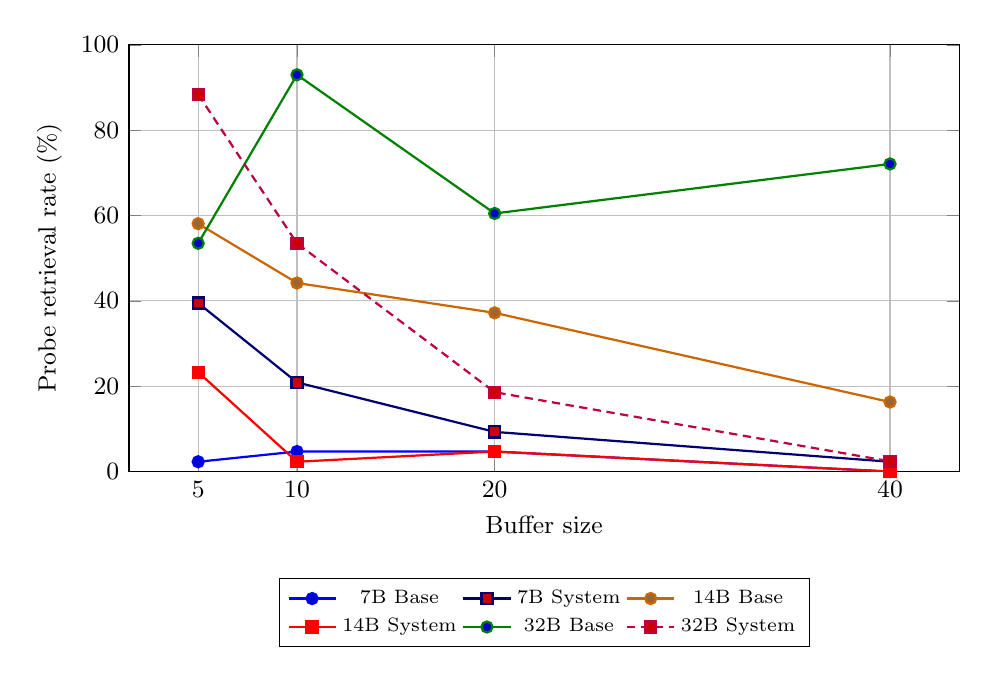
\begin{tikzpicture}
\begin{axis}[
width=\textwidth,
height=7cm,
xlabel={Buffer size},
ylabel={Probe retrieval rate (\%)},
xtick={5,10,20,40},
grid=both,
legend columns=3,
legend style={font=\scriptsize, at={(0.5,-0.25)}, anchor=north},
tick label style={font=\small},
label style={font=\small},
ymin=0,
ymax=100
]
\addplot+[color=blue, mark=*, thick] coordinates {(5,2.3) (10,4.7) (20,4.7) (40,0.0)};
\addlegendentry{7B Base}
\addplot+[color=blue!45!black, mark=square*, thick] coordinates {(5,39.5) (10,20.9) (20,9.3) (40,2.3)};
\addlegendentry{7B System}
\addplot+[color=orange!80!black, mark=*, thick] coordinates {(5,58.1) (10,44.2) (20,37.2) (40,16.3)};
\addlegendentry{14B Base}
\addplot+[color=red, mark=square*, thick] coordinates {(5,23.3) (10,2.3) (20,4.7) (40,0.0)};
\addlegendentry{14B System}
\addplot+[color=green!50!black, mark=*, thick] coordinates {(5,53.5) (10,93.0) (20,60.5) (40,72.1)};
\addlegendentry{32B Base}
\addplot+[color=purple, mark=square*, thick] coordinates {(5,88.4) (10,53.5) (20,18.6) (40,2.4)};
\addlegendentry{32B System}
\end{axis}
\end{tikzpicture}
\caption{RAG retrieval rate during the 43 recall probes. Probe retrieval is used as a memory-sufficiency signal because every probe asks the model to recover earlier topic content.}
\label{fig:probe_rag_buffer_all}
\end{figure}

Finally, Figure~\ref{fig:tpca_buffer_all} summarizes effective token efficiency. The system sometimes uses more raw input tokens, but it uses fewer tokens per correct answer in every tested setting. This is the key correction to the initial expectation: organized context is not always shorter, but it is more detailed.

\begin{figure}[htbp]
\centering
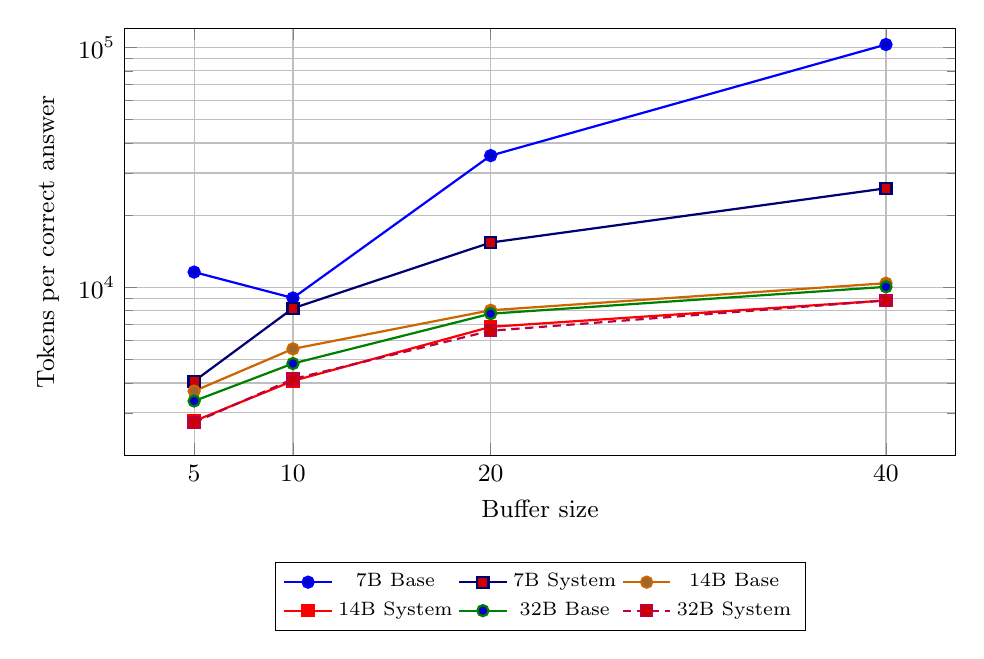
\begin{tikzpicture}
\begin{axis}[
width=\textwidth,
height=7cm,
xlabel={Buffer size},
ylabel={Tokens per correct answer},
xtick={5,10,20,40},
grid=both,
legend columns=3,
legend style={font=\scriptsize, at={(0.5,-0.25)}, anchor=north},
tick label style={font=\small},
label style={font=\small},
ymin=2000,
ymax=120000,
ymode=log
]
\addplot+[color=blue, mark=*, thick] coordinates {(5,11591.1667) (10,9038.0488) (20,35450.6531) (40,102923.4400)};
\addlegendentry{7B Base}
\addplot+[color=blue!45!black, mark=square*, thick] coordinates {(5,4067.4833) (10,8191.4196) (20,15389.0420) (40,25898.8558)};
\addlegendentry{7B System}
\addplot+[color=orange!80!black, mark=*, thick] coordinates {(5,3699.5890) (10,5547.5243) (20,8035.5215) (40,10418.1098)};
\addlegendentry{14B Base}
\addplot+[color=red, mark=square*, thick] coordinates {(5,2773.1043) (10,4079.3790) (20,6853.2095) (40,8825.9488)};
\addlegendentry{14B System}
\addplot+[color=green!50!black, mark=*, thick] coordinates {(5,3363.1150) (10,4819.4720) (20,7775.4519) (40,10059.6345)};
\addlegendentry{32B Base}
\addplot+[color=purple, mark=square*, thick] coordinates {(5,2737.7549) (10,4150.7460) (20,6600.2984) (40,8833.1696)};
\addlegendentry{32B System}
\end{axis}
\end{tikzpicture}
\caption{Tokens per correct answer across model sizes and buffer sizes. The y-axis uses a log scale because the 7B baseline becomes extremely inefficient at larger buffers.}
\label{fig:tpca_buffer_all}
\end{figure}

\section{Result Summary}\label{subsec:findings_summary}

The model-specific and cross-model results support five conclusions. First, branch-local context improves topic isolation across every tested model and buffer size. Second, the useful buffer range is model-dependent: 7B is safest at short buffers, 14B works best around $C=10$ or $C=20$, and 32B peaks at $C=20$. Third, recall probes show that the tree system preserves semantic topic content even when strict prefix-following fails. Fourth, recall-probe RAG is used as the retrieval diagnostic because each probe explicitly asks for old topic content, the model uese more retrieval when context is mixed or insufficient. Fifth, raw input-token count is not the main efficiency result; tokens per correct answer shows that Subchat Trees spends computation more productively as latency for Subchat System was lower.

These results motivate conversation trees as new interface adaption. A parent conversation can hold broad context, child nodes can isolate detailed follow-ups and sibling nodes can explore alternatives without contaminating one another. This matters for ordinary chat, multi-agent workflows and embodied systems where plans, observations, corrections and subgoals naturally form nested conversational state. Long context windows increase capacity, but they do not decide which prior turns belong to the current branch. Subchat Trees makes that structure explicit.
It provides more control to the user.
